%%%%%%%%%%%%%%%%%%%%%%%%%%%%%%%%%%%%%%%%%%%%%%%%%%%%%%%%%%%%%%%%%%%%%%%%%%%%%%%%%%%%%%%%%%%%%
%%									Chapitre 1											%
%%%%%%%%%%%%%%%%%%%%%%%%%%%%%%%%%%%%%%%%%%%%%%%%%%%%%%%%%%%%%%%%%%%%%%%%%%%%%%%%%%%%%%%%%%%%%
\chapter{An Overview of the Thesis}\label{chap:intro}
	\citationChap{
	The thing about quotes on the internet is that you can not confirm their validity
	}{Abraham Lincoln}
	\minitoc
	\newpage

%%%%%%%%%%%%%%%%%%%%%%%%%%%%%%%%%%%%%%%%%%%%%%%%%%%%%%%%%%%%%%%%%%%%%%%%%%%%%%%%%%%%%%%%%%%%%



% Début du chapitre

The purpose of this thesis is to provide a summary of the main research line of my PhD work carried out in between October 2017 and March 2021. During my PhD, I was hosted at the Inria Lille-Nord Europe (France) research center, in the SequeL team (now becomes Scool team). I was fortunate to be advised by Dr. Michal Valko, and also co-supervised by Dr. Emilie Kaufmann. The research thematic of SequeL lies in sequential decision making problems, to which all my contributions are devoted. In particular, this document mainly investigates sequential decision making in optimization problems.

\section{Context of the Thesis}\label{sec:intro.context}
	
%\subsection{What do we study and why?}\label{sec:intro.context.what}

Imagine that we dispose a numerical simulator for some complex task. Being considered as a black box, we can only get useful information by calling the simulator with different inputs. The goal is to find an input that optimizes the performance of the simulator. In the context of this thesis, we model such a scene as the so-called \gls{sequential optimization}\footnote{We thus do not consider parallelization in this thesis.} problem where a learner sequentially feeds inputs to a system/environment/function and from which they receive (deterministic or stochastic) feedback/payoffs/rewards/observations\footnote{Those terms can interchangeably employed.}. At some point, the learner shall be able to output a guess for the optimal input. Under some circumstances, a single call of the system is extremely costly. It is therefore of great interest to choose the input at each time step based on past observations.

Sequential optimization in a stochastic environment is an active research topic in both mathematics and computer science communities. For example,... Besides, it can also serve as an abstraction of many real-world problems in various fields such as finance~\citep{ziemba2010}, biology~\citep{durand2018contextual}, chemistry~\citep{floudas2000}, engineering~\citep{wang2007}, bioinformatics~\citep{moles2003}, etc. In this thesis, we are in particular interested in optimization of functions for which none (or few) regularity assumptions are made, and only noisy function evaluations can be observed. This is the \gls{go} or \gls{bbo} problem. Sometimes we can also refer to \gls{zo}, in contrast to \emph{first-order optimization} for which gradient-based information is available.

%Le problème de planification dans un Processus de Décision Markovien (MDP pour Markov Decision Process, [1]), pouvant modéliser la gestion de ressources dans un système de type smart grids ou encore le contrôle d'un robot, et celui de la construction d'intelligences artificielles pour des jeux, sont très liés à celui de l'optimisation séquentielle puisqu'ils reviennent à déterminer l'action qui dans un état donné maximise une fonction valeur, dont on peut obtenir des réalisations bruitées en explorant des trajectoires bien choisies.

%In this context, since one does not make extra regularity assumptions on the target function, one can imagine that it can be very costly to evaluate the function. Thus a good strategy for choosing adaptively the next observation is needed in order to find an optimal (or quasi-optimal) point with as few number of evaluations as possible. This is the sequential optimization problem. That being said, the main problematic of my thesis is the \emph{global sequential optimization} problem. Several applications could be investigated in this thesis, in particular the \emph{automatic hyper-parameter tuning} of machine learning algorithms~\citep{samothrakis2013,hoffman2014bayesgap,jamieson2016hyperband,li2017hyperband}.

Such optimization problem has been widely inspired by literature of~\gls{mab}. The original MAB problem is first studied by~\cite{thompson1933}, and can be described in the following way: A learner is given a set of $K$ arms $\{1,\ldots,K\}$ that follow $K$ unknown $[0,1]$-valued distributions $(\nu_k)_{1 \leq k \leq K}$, and a time horizon $n$. At each time step $t$, the process consists of (1) generating a vector of rewards $(r_{1,t} \sim \nu_1, \ldots, r_{K,t} \sim \nu_K)$, (2) picking an arm $k_t \in \{1,\ldots,K\}$ and (3) observing the reward $r_t = r_{k_t, t}$\footnote{Rewards of unchosen arms at time $t$ are not revealed, this partial feedback setting is a special case of the online learning with experts setting.}.

A natural observation is that, the learner needs to explore as many as possible to collect enough information, and in the mean time, they may also want to exploit the most profitable arm as much as possible. This trade-off is stated as the \gls{exploration-exploitation dilemma}. The usual performance criterion of the learner is measured by the total loss of the chosen arm at each time step w.r.t the best arm, namely the \emph{cumulative regret}. Typical good learners like \UCB~\citep{auer2002ucb} trade off between exploration and exploitation. In this thesis, we are particularly interested by another setting where the exploitation does not need to be performed at the same time as the exploration. In this context, it is natural to assess the learner in the same way as optimization problems. This setting, often named as \gls{bai}, is thus more strongly related to what we are to investigate in this thesis.

% 	\begin{tableth}
% 		\caption[Légende courte pour l'exemple de tableau]{Un tableau avec une légende tellement longue que ce serait hideux dans la liste des tableaux}
% 			\label{tab:exemple}
% 		\begin{tabular}{c|c}
% 			Coucou	& Au revoir\\
% 			\hline
% 			maman	& papa
% 		\end{tabular}
% 	\end{tableth}

% 	\begin{figureth}
% 		\begin{subfigureth}{0.4\textwidth}
% 			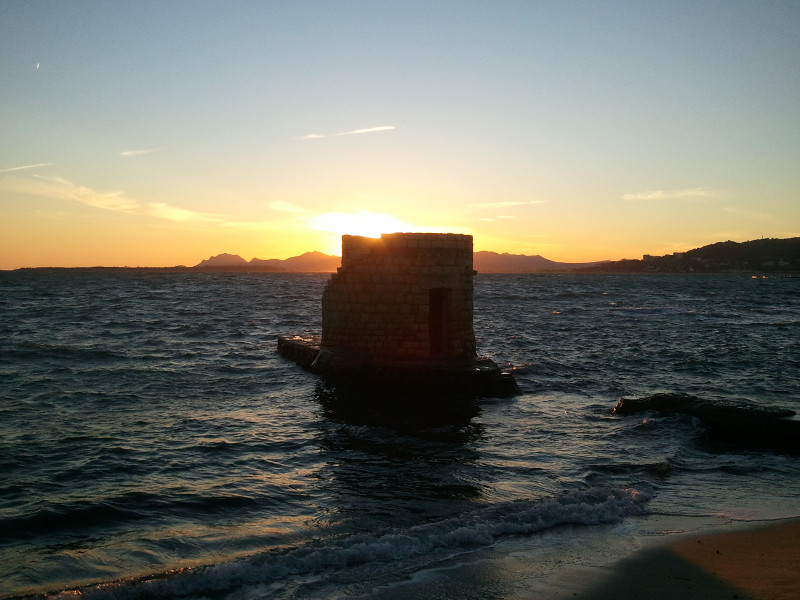
\includegraphics[width=\linewidth]{Chapter1/img/Antibes}
% 			\caption{Photo du Cap d'Antibes}
% 				\label{sub:Antibes}
% 		\end{subfigureth}
% 		\begin{subfigureth}{0.4\textwidth}
% 			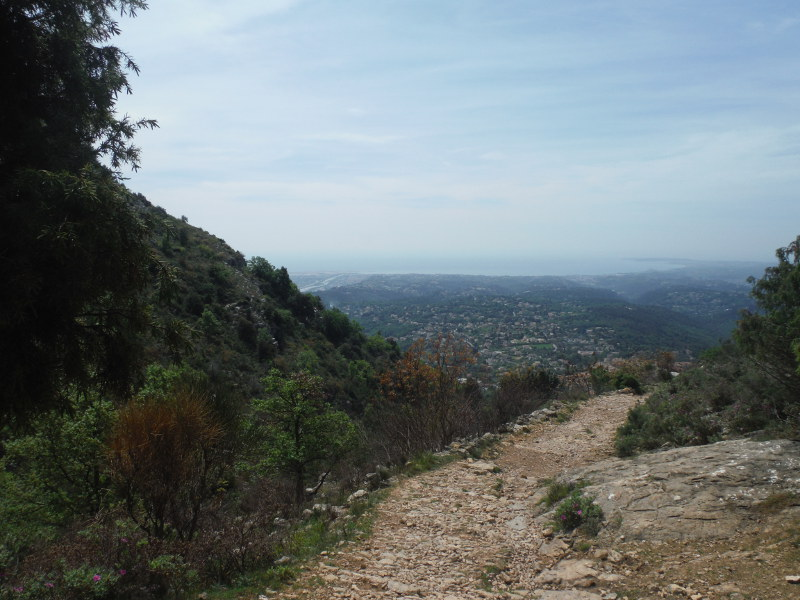
\includegraphics[width=\linewidth]{Chapter1/img/SaintJeannet}
% 			\caption{Saint Jeannet, depuis son Baou}
% 				\label{sub:SaintJeannet}
% 		\end{subfigureth}
% 		\caption[Légende courte pour la figure]{Exemple d'utilisation des sous-figures. J'utilise ici volontairement une légende longue.}
% 			\label{fig:exemple}
% 	\end{figureth}

\section{Multi-Armed Bandits and Optimization}\label{sec:intro.mab}
    
The research work presented in this dissertation tries to address sequential optimization problems under stochastic environments. A stochastic environment refers to an environment from which stochastic feedback are acquired when a data point is queried from the search/action space $\mathcal{X}$. Formally, we aim to maximise a target function $f:\mathcal{X}\rightarrow\mathbb{R}$, i.e. find 
\begin{equation}\label{eq:optim}
    \argmax_{x\in\mathcal{X}} f(x)\,.
\end{equation}

In its simplest form where the action space $\mathcal{X}$ is finite, the problem can be modeled as a \emph{stochastic multi-armed bandit}. The term \emph{bandit} is named, by analogy, after slot machines (or one-armed bandits) in a casino. A \emph{sequential decision making} problem comes up then when facing with several slot machines (multi-armed bandits). Concretely, a stochastic bandit is a collection of $K$ actions (also called arms) $\mathcal{X} = \{x_1,\ldots,x_K\}$. Each time the learner chooses one action $x_{a_t}\in\mathcal{X}$ which is then fed to the environment. The environment generates a reward $r_{a_t,t}=r_t$ which is assumed to be drawn from an unknown $[0,1]$-valued distribution $\nu_{a_t}$ and is revealed to the learner.

In its original formulation, the learning objective of a stochastic bandit is to maximise the total reward $\sum_{t=1}^T r_t$ obtained within a given time horizon $T$. In the literature of bandit, we usually denote by $\mu_k$ (resp. $\mu^\star$) the expectation of the unknown distribution $\nu_k$ (resp. the optimal arm), and the previous reward maximisation objective is equivalent to minimising the \emph{cumulative regret}: $T\mu^\star-\sum_{t=1}^T \mu_{a_t}$. %A such learning objective requires the learner to simultaneously acquire new information for potential future well-being (called \emph{exploration}), and optimize the current decision based on past observations (called \emph{exploitation}). 
Multi-armed bandits naturally addresses the trade-off between exploration and exploitation.

My PhD work, on the other hand, focuses on another learning objective which aims at identifying the optimal action, namely \emph{best-arm identification} (BAI). Contrary to regret minimisation, best-arm identification only cares about the exploration. Note that in this case, the time horizon $T$ is not necessarily known to the learner: we are often interested in finding the best arm with a given confidence level with as few queries as possible since in real applications function evaluations could be very expensive. This problem possesses many interesting variants and extensions that can all be formulated as the optimization problem~\eqref{eq:optim} to some extent, some of which will be covered in the next as I briefly describe some of the main contributions of my thesis.
    
    
\section{A Summary of the Contributions}\label{sec:intro.contributions}

\paragraph{Bayesian best-arm identification.} We begin by the vanilla BAI, for which the search space $\mathcal{X}$ is finite and one-dimensional and the target function $f$ can be considered as a function that maps each arm $x_k$ to its mean $\mu_k$. In one of our papers~\citep{shang2020t3c}, we employ some Bayesian machinery to address the problem based on the famous Thompson sampling (\TS). \TS is a Bayesian algorithm well known for regret minimization, for which it is now seen as a major competitor to the popular \UCB-typed approaches~\citep{auer2002ucb}. A natural question to ask is whether Bayesian methods can be also a good competitor to classical BAI approaches constructed upon complicated confidence intervals. However, it is well known that direct use of \TS cannot yield optimal performance for BAI and an adaptation such as \TTTS (top-two Thompson sampling) proposed by~\cite{russo2016ttts} is needed: by choosing between two different candidate arms in each round, it enforces the exploration of sub-optimal arms, which would be under-sampled by vanilla \TS due to its objective of maximizing rewards. \cite{shang2020t3c} provides further theoretical understandings of \TTTS and proposes a computational improvement \TCC with the same guarantees. \cite{shang2019dttts} also show that with some minor modifications, such Bayesian-flavored algorithms can be good candidates for applications like hyper-parameter optimization.

\paragraph{Extension to pure exploration for linear bandits.} A very natural and popular extension of the vanilla BAI is to take a finite space of features $\cX$ in $\R^d$ as the search space and consider a target function $f$ that maps each arm $\mathbf{x}$ (also called context in this case) to its linear combination with a \emph{regression parameter} $\btheta$, and is thus called linear bandits. $\btheta$ is of course unknown to the learner. Previous work on this topic were not (asymptotically) optimal. A lower bound, which can be written as a complicated minimax optimization problem, is given by~\cite{garivier2016tracknstop}. In a subsequent work, we develop a saddle-point approach to that lower bound optimization problem, which then led to optimal algorithms for linear BAI in the fixed-confidence regime~\citep{degenne2020game}. In addition, their empirical performance is competitive with the best existing algorithms. We also investigate a natural adaptation of our Bayesian approaches developed in the previous paper~\citep{shang2020t3c}. Unfortunately, they do not seem to be (asymptotically) optimal (work not published yet). Therefore, knowing whether one can find an *optimal* Bayesian approach remains an open problem.

\paragraph{Infinitely-armed bandits and black-box optimization.} Finally, a more general problem is to consider an infinite (probably uncountable) measurable space $\mathcal{X}$, and each arm $x\in\mathcal{X}$ gets its mean reward $f(x)$ through the reward function $f$. We study the noisy setting in which the obtained reward is a noisy evaluation of $f: r_t = f(x_t) + \epsilon_t$. This problem is also better known under the name \emph{black-box optimization}, to which the main approaches include Bayesian optimization~\citep{brochu2010bayesian}, evolutionary algorithms and hierarchical bandits~\citep{bubeck2010x}. We opt for another performance measure in this case, namely the simple regret: $\max_{x\in\mathcal{X}} f(x) - f(x_{j_t})$ with $x_{j_t}$ our guess at time $t$. In a recent work of ours, we provide a general wrapper for hierarchical bandit algorithms that only have guarantees for their simple regret~\cite{shang2019adaptive}. We show that with a cross-validation scheme, any hierarchical bandit algorithm with simple regret guarantees can be plugged into our meta-algorithm with only a tiny increase in the resulting simple regret.

\paragraph{Included in this thesis}

\cite{shang2018adaptive,shang2019dttts,shang2019adaptive,shang2020dttts,degenne2020game,shang2020t3c}.

\paragraph{Not included in this thesis}

\cite{shang2020vector,shang2021safe,menard2021ucbmq}.

\cite{rlberry2021}.

\section{Organization of the Thesis}\label{sec:intro.organization}

% \newpage
% \bibliographystyle{plain}
% \bibliography{library}
